\documentclass[aspectratio=169,t]{beamer}

% ---------------------
% General settings
% ---------------------

% Remove the navigation elements
\setbeamertemplate{navigation symbols}{}

% Import Packages
\usepackage[utf8]{inputenc}
\usepackage[T1]{fontenc}
\usepackage{amsmath,amssymb}
\usepackage{graphicx}
\usepackage{listings}
\usepackage{tikz}
\usepackage{animate}
\usepackage{hyperref}
\usepackage{adjustbox}
\usepackage{xcolor}

% Define Helvetica as default font 
% (I don`t like the default font - remove this if you are of other opinion)
\usepackage[scaled=0.95]{helvet}
\renewcommand{\familydefault}{\sfdefault}

% Enable semi-transparent animation preview
\setbeamercovered{transparent}

% ---------------------
% Timer settings
% ---------------------

% Define duration (in minutes)
\def\duration{90}

% Lengths
\newlength{\outerradius}
\newlength{\innerradius}
\newlength{\boundarybox}
\newlength{\textboundary}
\setlength{\outerradius}{2cm}
\setlength{\innerradius}{1.5cm}
\setlength{\boundarybox}{3cm}
\setlength{\textboundary}{3cm}

% Colors
\definecolor{background}{RGB}{255, 255, 255}
\definecolor{mainfont}{HTML}{414851}
\definecolor{secondaryfont}{HTML}{C9D0D5}
\definecolor{timeleft}{HTML}{89B2BB} 
\definecolor{timepassed}{HTML}{E4E8E2} 
\definecolor{timeelapsed}{HTML}{EDDFDB}

% Functions
\newcommand{\hours}[1]{\pgfmathparse{(int(floor(#1/3600)))/100}\pgfmathprintnumber[skip 0.=true, dec sep={}, fixed, fixed zerofill, precision=2]\pgfmathresult}
\newcommand{\minutes}[1]{\pgfmathparse{(int(floor((#1/60)-(floor(#1/3600)*60))))/100}\pgfmathprintnumber[skip 0.=true, dec sep={}, fixed, fixed zerofill, precision=2]\pgfmathresult}

\begin{document}
\begin{frame}{}
	\begin{center}
		\begin{animateinline}[controls={play, stop, step}, autoplay, poster=first]{0.01666667}
			\multiframe{\duration}{n=0+60}{
				\begin{tikzpicture}
					% Macros
					\pgfmathsetmacro{\timeleft}{(\duration*60)-\n}
					\pgfmathsetmacro{\percentage}{\timeleft/(\duration*60)*100}
					\pgfmathsetmacro{\angle}{\timeleft/(\duration*60)*360}

					% Boundary box
					\fill[background] (-\boundarybox,-\boundarybox) rectangle (\boundarybox,\boundarybox);

					% Progress indicating circle
					% Lower layer circle (representing time passed)
					\fill[timepassed] (0,0) circle (\outerradius);

					% Middle layer circle (representing time left)
					\fill[timeleft] (0,0) -- (90:\outerradius) arc (90:\angle+90:\outerradius) -- cycle;

					% Upper layer circle (freeing up space within the outer circle for text)
					\fill[background] (0,0) circle (\innerradius);

					% Text
					% Text within the progress indicating circle
					% Header
					\node[text width=\textboundary,align=center] at (0,0.5) {\small \textcolor{secondaryfont}{Time left:}};
					% Time left
					\node[text width=\textboundary,align=center] at (0,0) {\LARGE \textcolor{mainfont}{\hours{\timeleft}h \minutes{\timeleft}min}};
					% Total time
					\node[text width=\textboundary,align=center] at (0,-0.5) {\large \textcolor{secondaryfont}{\hours{\duration*60}h \minutes{\duration*60}min}};

					% Text below the progess indicating circle
					\node at (0,-2.5) {\textcolor{secondaryfont}{Controls:}};
				\end{tikzpicture}
			}
			\newframe[1]
			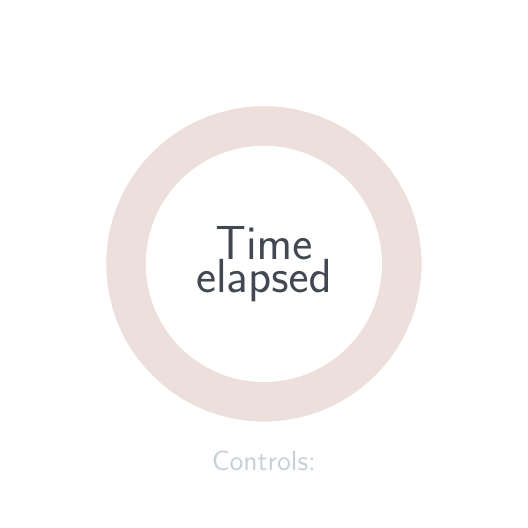
\begin{tikzpicture}
				% Boundary box
				\fill[background] (-\boundarybox,-\boundarybox) rectangle (\boundarybox,\boundarybox);

				% Progress indicating circle
				% Lower layer circle (representing time passed)
				\fill[timepassed] (0,0) circle (\outerradius);

				% Middle layer circle (representing time left)
				\fill[timeelapsed] (0,0) -- (0, \outerradius) arc (90:90-3.6*100:\outerradius) -- (0,0);

				% Upper layer circle (freeing up space within the outer circle for text)
				\fill[background] (0,0) circle (\innerradius);

				% Text
				% Text within the progress indicating circle
				% Header
				\node[text width=\textboundary,align=center] at (0,0) {\LARGE \textcolor{mainfont}{Time \\elapsed}};

				% Text below the progess indicating circle
				\node at (0,-2.5) {\textcolor{secondaryfont}{Controls:}};
			\end{tikzpicture}
		\end{animateinline}
	\end{center}
\end{frame}
\end{document}
